\documentclass{report}

\usepackage{polski} % Pozwala na użycie polskiego. Ustawia między innymi fontenc na T1
\usepackage[utf8]{inputenc} % Informuje o kodowaniu

\usepackage{xcolor}% http://ctan.org/pkg/xcolor
\definecolor{LinkColor}{HTML}{1d5cc1} % Kolor do linków
\usepackage{hyperref}% http://ctan.org/pkg/hyperref

\definecolor{LinkColor}{HTML}{1d5cc1}

\usepackage{tabto}

\usepackage{graphicx} % Pakiet do obrazów
\graphicspath{ {./Obrazy/} } % Folder, z którego będą brane obrazy
\usepackage{float} % Dodatkowe pozycjonowanie obrazów - [H]
\usepackage{subcaption} % Kilka obrazów w jednej figurze

% Nie twórz nowych stron
\usepackage{etoolbox}
\makeatletter
% \patchcmd{\chapter}{\if@openright\cleardoublepage\else\clearpage\fi}{}{}{}
\makeatother

\title{Specyfikacja funkcjonalna -- Wireworld}
\author{Krzysztof Dąbrowski i Jakub Bogusz}
\date{\today}

\begin{document}
\maketitle{}

\tableofcontents{}

\chapter{Cel projektu}
Celem projektu jest implementacja automatu komórkowego Wire World w języku Java z interfejsem graficznym zaimplementowanym przy pomocy biblioteki JavaFX. Gotowy program ma pozwalać użytkownikowi przeprowadzać symulacje zgodne z określonymi zasadami. Parametrami generacji użytkownik będzie mógł sterować ręcznie przy pomocy graficznego \hyperref[sec:wyglad-gui]{\textcolor{LinkColor}{interfejsu użytkownika}}.

Interfejs będzie wyświetlał na bieżąco podgląd kolejnych generacji. Użytkownik będzie miał możliwość wstrzymania symulacji oraz zmianę stanu planszy przy pomocy narzędzi edycji.

Ponadto będzie istnieć również możliwość przełączenia trybu symulacji z Wire World na automat komórkowy Game of life.

\chapter{Opis ogólny problemu}

\section{Wstęp}
Projekt skupia się na realizacji 3 głównych aspektów problemu. Będą to odpowiednio automaty komórkowe ,,Game of Life'' i ,,Wireworld'' oraz wizualna prezentacja działania tych automatów. 

\section{Wire World}

Wire World jest automatem komórkowym wymyślonym przez Briana Silvermana w roku 1987.  Jest często używany do symulacji elementów elektronicznych operujących na wartościach bitowych. Pomimo prostoty reguł, jakie nim rządzą, za pomocą Wireworld można nawet stworzyć działający komputer.

\subsection{Symulacja}
\begin{minipage}{\textwidth} %Akapit ma być na jednej stronie
    \paragraph{Stany}  Komórka może znajdować się w jednym z czterech stanów:
    \begin{itemize}
    \item pusta,
    \item głowa elektronu,
    \item ogon elektronu,
    \item przewodnik.
    \end{itemize}
\end{minipage}

\paragraph{Pokolenie} to zbiór stanów wszystkich komórek w danej chwili. Gdy stan pokolenia jest ustalony, możliwe jest utworzenie nowego (potomnego) pokolenia komórek, powstających według poniższych zasad.

\paragraph{Reguły} Następne pokolenie generowane jest zgodnie z regułami:
\begin{itemize}
\item Jeżeli komórka jest pusta, to pozostaje pusta niezależnie od jej otoczenia,
\item Jeżeli komórka jest głową elektronu, to zmieni się w ogon elektronu,
\item Jeżeli komórka jest ogonem elektronu, to zmieni się w przewodnik,
\item Jeżeli komórka jest przewodnikiem i sąsiaduję z jedną lub dwoma komórkami będącymi głowami elektronu, to zmieni się w przewodnik.
\end{itemize}

\subsection{Struktury}
Symulacja przeprowadzona zgodnie z powyższymi regułami może prowadzić do powstania ciekawych obiektów zwanych strukturami. 
\begin{figure}[h]
\centering
\setlength{\fboxsep}{0pt} %Odstęp 0
\setlength{\fboxrule}{1pt} %Grubość ramki 1p
\fbox{\includegraphics[width=8cm]{Obrazy/struktury_w.png}}
\caption{Przykłady struktur - dioda przewodząca i nieprzewodząca}
\end{figure}


\section{Game of life}

Game of life jest automatem komórkowym wymyślonym przez brytyjskiego matematyka John Horton Conway
w 1970 roku. Polega na symulacji kolejnych pokoleń życia komórek według następujących zasad.

\subsection{Symulacja}

\paragraph{Stany}  Komórka może znajdować się w jednym z dwóch stanów:
\begin{itemize}
\item żywa,
\item martwa.
\end{itemize}

\paragraph{Pokolenie} to stan wszystkich komórek w danej chwili. Gdy stan pokolenia jest ustalony, możliwe jest utworzenie nowego (potomnego) pokolenia komórek, powstających według poniższych zasad.

\paragraph{Reguły} Następne pokolenie generowane jest zgodnie z regułami:
\begin{itemize}
\item Jeżeli komórka była martwa i miała dokładnie 3 żywych sąsiadów, w następnym pokoleniu staje się żywa,
\item Jeżeli komórka była żywa to pozostaje żywa jeśli miała dwóch lub trzech żywych sąsiadów. W przeciwnym razie staje się martwa.
\end{itemize}

\subsection{Struktury}
Symulacja przeprowadzona zgodnie z powyższymi regułami może prowadzić do powstania ciekawych obiektów zwanych strukturami. 

\begin{figure}[h]
\centering
\setlength{\fboxsep}{0pt} %Odstęp 0
\setlength{\fboxrule}{1pt} %Grubość ramki 1p
\fbox{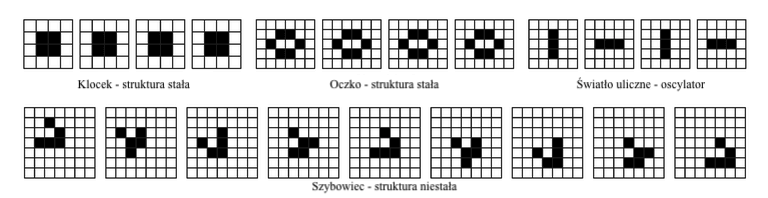
\includegraphics[width=13cm]{Obrazy/struktury.png}}
\caption{Przykłady struktur}
\end{figure}

Reguły symulacji umożliwiają również tworzenie dużo bardziej skomplikowanych struktur (jak na przykład maszyna Turinga -- https://youtu.be/My8AsV7bA94).

\section{Interfejs użytkownika}
\label{sec:opis-interfejs}
Ważnym aspektem programu jest sposób interakcji z użytkownikiem.
Realizowana aplikacja będzie obsługiwana poprzez graficzny interfejs użytkownika.

Interfejs pozwoli na poniższe funkcjonalności:
\begin{itemize}
    \item Bieżący podgląd stanu symulacji,
    \item Możliwość dostosowania prędkości symulacji,
    \item Zapis aktualnego pokolenia do pliku,
    \item Wyczytanie pokolenia z pliku,
    \item Edycje poszczególnych komórek w trakcie symulacji,
    \item Wstawianie figur wybranych z przybornika.
\end{itemize}

\chapter{Działanie programu}

\section{Opis komunikacji z użytkownikiem}
Po uruchomieniu programu zostanie wyświetlony graficzny interfejs, który pozwoli użytkownikowi sterować parametrami w dowolny sposób, zgodny z regułami symulacji. W razie wystąpienia błędów program będzie informować użytkownika wyświetlając nowe okno zawierające opis błędu.

W ramach interfejsu użytkownik będzie mógł wykonywać czynności opisane w punkcie \ref{sec:opis-interfejs}{} oraz przełączać między automatami Game of Life i Wire World.

\section{Wygląd interfejsu użytkownika} \label{sec:wyglad-gui}
Interfejs użytkownika będzie wyglądał jak poniżej. Wyszczególnione obszary są zaznaczone numerami.
\begin{figure}[H]
    \centering
    \includegraphics[width=0.99\columnwidth]{gui.png} %Dla 1 nie mieści się na tej samej stronie
    \caption{Całokształt interfejsu użytkownika}
\end{figure}

\section{Opis elementów}
\paragraph{1 Podgląd aktualnego stanu symulacji} \mbox{} \\
W tej części będzie wyświetlane bieżące pokolenie symulacji aktualnego automatu komórkowego. Po bokach panelu znajduje się \textbf{suwak} pozwalające na zmianę oglądanego obszaru planszy.

\paragraph{2 Ustawienia symulacji i planszy} \mbox{} \\
Sekcja kontrolek umożliwiających sterowanie symulacją oraz zmianę całości planszy.

Po lewej stronie znajduje się grupa elementów wpływających bezpośrednio na podgląd symulacji.
\begin{itemize}
    \item Play -- uruchamia automatycznie przechodzenie między staniami symulacji,
    \item Stop -- zatrzymuje automatycznie przechodzenie między staniami symulacji,
    \item Speed -- zmienia tempo automatycznego przechodzenie między staniami symulacji,
    \item Next generation -- ręczne przejście do następnego stanu symulacji,
    \item Zoom -- zmienia skalę podglądu aktualnego stanu,
    \item Speed -- zmienia prędkość przechodzenia między kolejnymi stanami symulacji.
\end{itemize}

Po prawej stronie umieszczona jest grupa elementów pozwalających na reset całego stanu planszy.
\begin{itemize}
    \item Grid height, Grid height -- wprowadzenie rozmiaru planszy jaka zostanie utworzona,
    \item Create -- Tworzy plansze o podanym rozmiarze, gdy plansza już istnieje i podany rozmiar jest równy planszy już istniejącej, opis 			przycisku zamienia się na "Clear", i wciśnięcie go zmienia stan wszystkich komórek na "Pusty" w przypadku WireWorld lub "Martwy" w 		przypadku Game of Life,
    \item Random -- Nadanie wszystkim komórkom losowych stanów,
\end{itemize}

\paragraph{3 Przybornik} \mbox{} \\
Boczny przybornik zawierał będzie dwie zakładki, które będą pozwalały na edycje fragmentów planszy.

\begin{figure}[H]
    \centering
    \begin{subfigure}[b]{0.49\textwidth}
        \centering
        \includegraphics[width=0.4\textwidth]{przybornik1}
        \caption{Przybornik Cells}
    \end{subfigure}
    \begin{subfigure}[b]{0.49\textwidth}
        \centering
        \includegraphics[width=0.4\textwidth]{przybornik2}
        \caption{Przybornik External}
    \end{subfigure}
\end{figure}

Zakładka \textbf{Cells} umożliwi wybranie stanu komórki, a następnie nadanie komórkom wybranego stanu poprzez klikanie myszą komórek w oknie podglądu.

Zakładka \textbf{External} da dostęp do zestawu gotowych figur, które użytkownik będzie mógł wstawić w wybranym miejscu planszy. Użytkownik będzie mógł dodać własne figury do przybornika oraz zapisać i wczytać stan całej planszy przy pomocy guzików z tej zakładki.

\paragraph{4 Wybór automatu} \mbox{} \\
Wstążka pozwalająca na zmianę aktywnego automatu komórkowego.

\section{Stany interfejsu}
Podczas korzystania z aplikacji interfejs będzie ulegał drobnym zmianom (głównie elementy odpowiadające za aktualnie niedostępne opcje będą zmieniać kolor na szary).

\subsection{Po włączeniu programu}
Większość kontrolek jest \textbf{wyłączonych} do momentu wczytania planszy z pliku lub wygenerowania losowej. Program domyślnie wyświetla okno symulacji automatu Wire World.

\begin{figure}[H]
    \centering
    \includegraphics[width=\textwidth]{gui-initial}
    \caption{Stan interfejsu po uruchomieniu aplikacji}
\end{figure}

\subsection{W trakcie symulacji}
Można zmienić tempo symulacji oraz wstrzymać generację następnych pokoleń.

\begin{figure}[H]
    \centering
    \includegraphics[width=\textwidth]{gui-running}
    \caption{Stan interfejsu w trakcie symulacji}
\end{figure}

\subsection{Symulacja wstrzymana}
Możliwe jest edytowanie komórek przy pomocy narzędzia oraz wstawianie figur.

\begin{figure}[H]
    \centering
    \includegraphics[width=\textwidth]{gui-paused}
    \caption{Stan interfejsu przy wstrzymanej symulacji}
\end{figure}

\section{Tryb automatu Game of Live}
Program obsługuje również automat komórkowy Game of Life. Przełączenie między aktualnym automatem jest realizowane przy pomocy wstążki na górze interfejsu.
Większość elementów interfejsu pozostanie taka sama jak w automacie Wire World. Inaczej będzie wyglądał przybornik do edycji planszy, ponieważ automat ten zawiera inne stany komórek.

\chapter{Edycja planszy}
Użytkownik ma kilka możliwości na wgranie planszy do programu lub edycję już istniejącej. Są one wymienione poniżej.

\section{Plik wejściowy}  \label{format}
Program pozwala na wczytanie całego stanu planszy (wraz z rozmiarem) z pliku. Dzięki temu możliwe jest łatwe odtworzenie stanu ze wcześniejszej symulacji lub prezentacja skomplikowanego układu.

Program będzie w stanie obsłużyć różnie formaty plików wymienione poniżej.

\subsection{Plansza w formacie JSON}
W celu nadania danym przenośności, oraz ułatwienia generacji danych przy pomocy zewnętrznych narzędzi zostanie wykorzystany format JSON. Jest to \textbf{domyślny format} zapisu planszy.

\subsubsection{Przykład}
Przykład zapisu przedstawionej planszy. 

\begin{figure}[H]
    \centering
    
\includegraphics[height=4cm]{przyklad-planszy-wireworld}
    \caption{Przykładowa plansza}
\end{figure}

\noindent{}Plik reprezentujący planszę:
\begin{verbatim}
{
  "width" : 2,
  "height" : 3,
  "states" : [ "HEAD", "TAIL", "HEAD", "HEAD", "HEAD", "EMPTY" ]
}
\end{verbatim}

Wartości \texttt{width} i \texttt{height} określają wymiary planszy.
\texttt{states} zawiera tablicę reprezentującą poszczególne stany komórek w kolejności od lewej do prawej oraz od góry do dołu. 

\subsection{Plansza w formacie XML}
Możliwy jest również zapis stanu planszy do pliku XML. Z uwagi na mniejszą czytelność oraz większy rozmiar plików tego typu, nie jest to domyślnie używany format. Użytkownik będzie miał możliwość zmiany formatu pliku, do jakiego chce zapisać planszę przy pomocy interfejsu graficznego.

\subsubsection{Przykład}
Przykład zapisu przedstawionej planszy. 

\begin{figure}[H]
    \centering
    
\includegraphics[height=4cm]{przyklad-planszy-wireworld}
    \caption{Przykładowa plansza}
\end{figure}

\begin{samepage}
\noindent{}Plik reprezentujący planszę:
\begin{verbatim}
<Board>
  <width>2</width>
  <height>3</height>
  <states>
    <states>CONDUCTOR</states>
    <states>HEAD</states>
    <states>TAIL</states>
    <states>TAIL</states>
    <states>CONDUCTOR</states>
    <states>EMPTY</states>
  </states>
</Board>
\end{verbatim}
\end{samepage}
Wartości \texttt{width} i \texttt{height} określają wymiary planszy.
\texttt{states} zawiera tablicę reprezentującą poszczególne stany komórek w kolejności od lewej do prawej oraz od góry do dołu.

\section{Przybornik stanów}
Jedną z części interfejsu użytkownika będzie przybornik pozwalający na wybór jednego ze stanów aktualnego automatu komórkowego. Po zaznaczeniu jednego ze stanów użytkownik będzie miał możliwość zamiany wybranych komórek aktualnego pokolenia na wybrany stan.

\section{Wstawianie figur}
Interfejs będzie zawierał zestaw typowych figur dla aktualnego automatu komórkowego. Możliwe będzie zaznaczenie wybranej figury oraz wstawienie jej w wybrane miejsce symulacji planszy.

Użytkownik będzie mógł wybrać figurę z listy figur. Następnie po kliknięciu wybranego pola planszy figura zostanie wstawiona w to miejsce, tak by lewy górny róg figury znalazł się w wybranym miejscu.

\subsection{Rozszerzanie listy figur}
Użytkownik będzie miał możliwość dodania własnych figur do domyślnej listy.
Interfejs będzie zawierał przycisk wywołujący edytor pojedynczej figury. Po wywołaniu edytora użytkownik będzie mógł narysować własną figurę, która po zatwierdzeniu zostanie dodana do listy.
Figury rozszerzające podstawową listę będą zapisywanie w pliku konfiguracyjnym. Dzięki temu po uruchomieniu programu zostaną one ponownie załadowane. 

\section{Zapis stanu planszy}
Program będzie w stanie zapisać aktualny stan planszy w formacie, który umożliwi późniejsze wczytanie planszy. Użytkownik będzie miał możliwość wyboru formatu pliku do jakiego chce zapisać stan.

\section{Wczytanie stanu planszy}
Program będzie w stanie wczytać stan planszy z pliku wskazanego przez użytkownika. Typ pliku zostanie rozpoznany po rozszerzeniu pliku.

\chapter{Sytuacje wyjątkowe}
Czasem działanie programu może ulec zmianie na skutek nieprawidłowych danych wejściowych, niestandardowych ustawień wprowadzonych przez użytkownika lub z przyczyn losowych. Ten rozdział opisuje jak program zachowa się w takiej sytuacji, oraz co może ją wywołać.

\section{Zmiana działania programu}
W wyjątkowych sytuacjach działanie programu może ulec drobnym zmianom.

\paragraph{Nieoptymalna postać liczby}
Jeśli użytkownik wprowadzi liczbę o dłuższej postaci niż jest to koniecznie, po zatwierdzeniu pola liczba zostanie skrócona do optymalnej długości.

Na przykład po wprowadzeniu 00034 jako wysokość planszy, po zakończeniu edycji pola wartość ta zostanie zmieniona na 34.

\section{Błędy}
Opis błędów, które mogą wystąpić w trakcie działania programu. Komunikaty ich dotyczące będą wyświetlane w nowych oknach zawierających ich treść.

\subsection{Błędy pliku wejściowego}

\paragraph{Pusty plik}
W przypadku gdy plik wskazany przez użytkownika będzie pusty program powiadomi go o tym i nie wczyta planszy.

\paragraph{Rozmiar planszy nie będący liczbą}
Jeśli w miejscu rozmiaru planszy (szerokości lub wysokości) znajdować się będą wartości inne niż liczby, liczby ujemne lub liczby których iloczyn jest większy niż 1 000 000 program nie wczyta rozmiaru planszy. W takiej sytuacji wyświetli odpowiedni komunikat i nie wczyta planszy.
 
 \paragraph{Niezgodności rozmiaru planszy z faktycznym stanem}
 Jeśli podany rozmiar planszy nie będzie się zgadzać z ilością podanych w nim stanów komórek, program wyświetli odpowiedni komunikat i nie wczyta planszy.
 
 \paragraph{Nieprawidłowy znak w pliku}
 Jeśli podczas czytania pliku program napotka nierozpoznawany znak, wyświetli odpowiedni komunikat i nie wczyta planszy.
 
 \paragraph{Błąd składniowy}
 Jeśli plik będzie zawierał błąd składniowy (w formatowaniu JSON lub XML), program wyświetli odpowiedni komunikat i nie wczyta planszy.
 
\subsection{Błędy podczas używania GUI}
\paragraph{Zły rozmiar planszy}
Jeśli użytkownik w polu przeznaczonym na rozmiar planszy spróbuje wpisać:
\begin{itemize}
	\item znaki nie będące cyframi,
	\item wartość mniejszą lub równą 0,
	\item wartości zbyt duże (liczba komórek przekraczająca 1 000 000)
\end{itemize}
to pole nie zmieni wartości.

Na przykład po próbie wpisania ciągu znaków znaków ,,52e4'' jako szerokość planszy pole będzie zawierało kolejno wartości: 5, 52, 52, 524. Nieprawidłowy znak zostanie zignorowany.

\paragraph{Zły format wczytywanego pliku}
Jeśli program nie obsługuję wczytywania wybranego formatu pliku to powiadomi o tym użytkownika odpowiednim komunikatem w którym  przedstawi mu również obsługiwane typy plików wejściowych.

\paragraph{Brak miejsca na figurę}
Jeśli użytkownik spróbuje wstawić figurę w miejsce na planszy, tak, że cała figura nie zmieści się na aktualnej planszy figura nie zostanie wstawiona oraz zostanie wyświetlony komunikat o błędzie.

\subsection{Błędy losowe}
\paragraph{Brak pamięci operacyjnej}
Gdyby w systemie zabrakło pamięci program nie będzie w stanie funkcjonować poprawnie. Program wyświetli komunikat o błędzie i przerwie symulację. Następnie poprosi o próbę wczytania mniejszej planszy lub uruchomienia programu później.

\end{document}
